% This is a template to create your midterm report as a pdf.
% Just fill in the areas and run pdflatex
% For more information on LaTeX documents consult The (Not So
% Short Introduction to LateX2e
%
% to compile your report use the command
% pdflatex finalreport.tex
%
% if you have \ref useage or other cross links
% you will have to run the above command again

% set 12pt font
\documentclass[12pt]{article}
% some useful packages
\usepackage[pdftex]{graphicx,color}
\usepackage{fullpage}
\usepackage{setspace}
\usepackage{etoolbox}
\apptocmd{\sloppy}{\hbadness 10000\relax}{}{}
\def\baselinestretch{1.5} % line spaceing
\def\arraystretch{1.5} % table padding
% set title
\title{Final Design Report \\
	ECE 437L}
% fill in the blanks
\author{Yutong Huang, Yiheng Chi \\
        John Skubic, Noah Chesnut, Abhishek Srikanth}
% \today will put todays date
% or you can manually put the date in
\date{Apr. 28, 2017}
% cover page is a page by itself

\begin{document}
  \maketitle

  \newpage
% executive overview remember
% this should be on a page by itself
  \section{Executive Overview}

  At the end of semester, pipeline processor design, pipeline processor with caches design, and multicore design have all been completed and carefully verified. In this report, we are going to compare pros and cons of each design including frequency, instruction CPI, total instruction execution time, and resource requirement. For controlling variables, comparison is performed under the same binary program which perform a merge sort algorithm. The only difference is that multicore processor is run with multi-core version mergesort. Merge sort is selected since it contains a lot of branch instructions, heavy dependency of each instruction, and frequent load use. Besides, RAM latency with 6 cycles is selected to differentiate the design with and without caches.\\
  In general, design with less modules uses less resources, since caches need a lot of registers to store data and some logics to control read and write, coherence. Multicore even doubles everything, making the whole design resource usage 4 times larger than pure pipeline design. Also, because of complex combinational control logic for cache controller and memory controller, the maximum clock speed is way slower than pure pipeline design; multicore design has only half of clock speed comparing to pipeline design; thus, the latency of single instruction is slower in cache and multicore design. However, locality eliminates a lot of memory read and write, saving about ⅔ of execution cycles. In total, based on testing result, pipeline design with caches will execute program much faster than pure pipeline design and consume more resources simultaneously, but multicore design with really slow clock rate executes program even slower than pipeline design with caches although less clock cycles are used.

  \newpage
  \section{Processor Design}

% Uncomment after you create the block diagram graphic.
% Figure 1. Block Diagram of Pipeline Processor Design
  \begin{figure}[hbp!]
    \begin{center}
      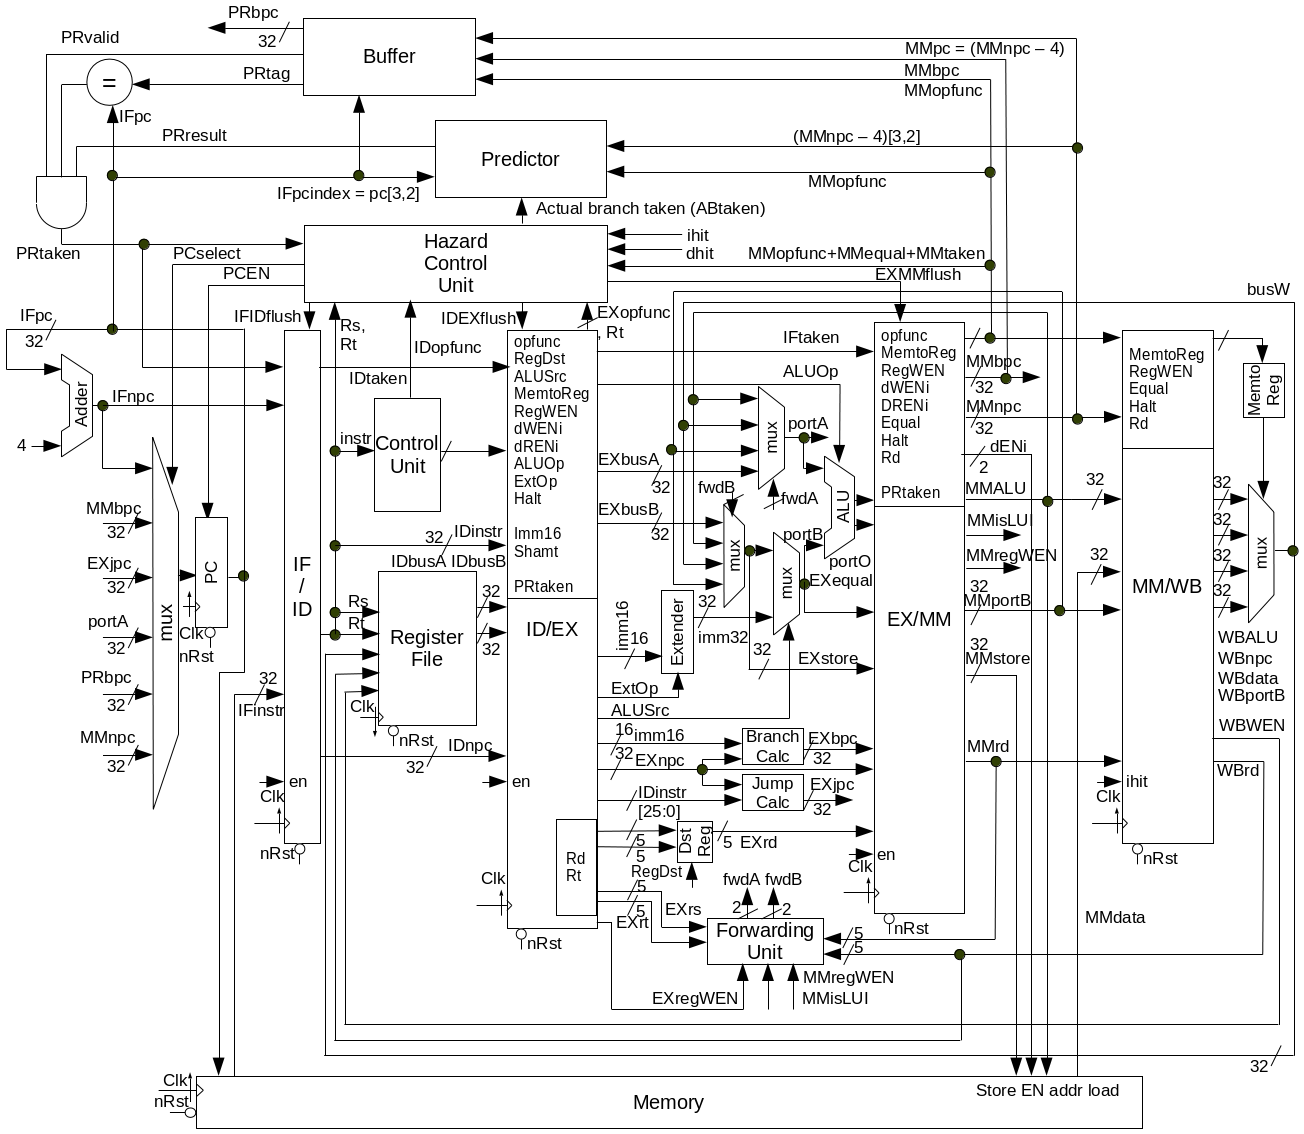
\includegraphics[width=\textwidth]{diagrams/diagram_pipeline.png}
    \end{center}

    \caption{Pipeline Block Diagram}
		\label{fig:pipeline}
  \end{figure}

% Figure 2. Block Diagram of Instruction Cache
  \newpage
  \begin{figure}[hbp!]
    \begin{center}
      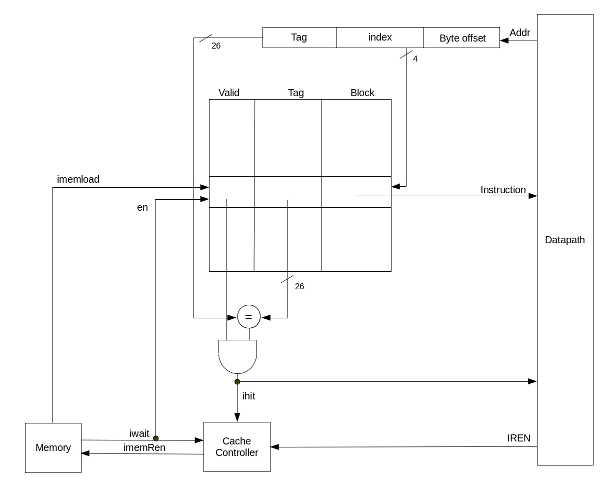
\includegraphics[width=.8\textwidth]{diagrams/diagram_icache.png}
    \end{center}

    \caption{Instruction Cache Block Diagram}
		\label{fig:icache}
  \end{figure}

% Figure 3. State Diagram of Instruction Cache
  \begin{figure}[hbp!]
    \begin{center}
      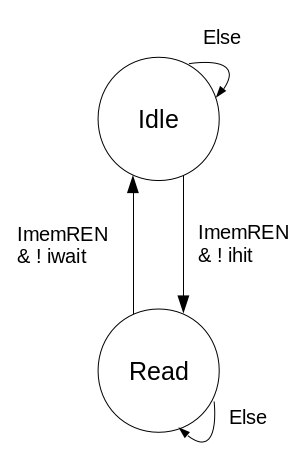
\includegraphics{diagrams/icache_state_machine.png}
    \end{center}

    \caption{Instruction Cache State Diagram}
		\label{fig:icache_sd}
  \end{figure}

% Figure 4. Block Diagram of Data Cache
  \newpage
  \begin{figure}[hbp!]
    \begin{center}
      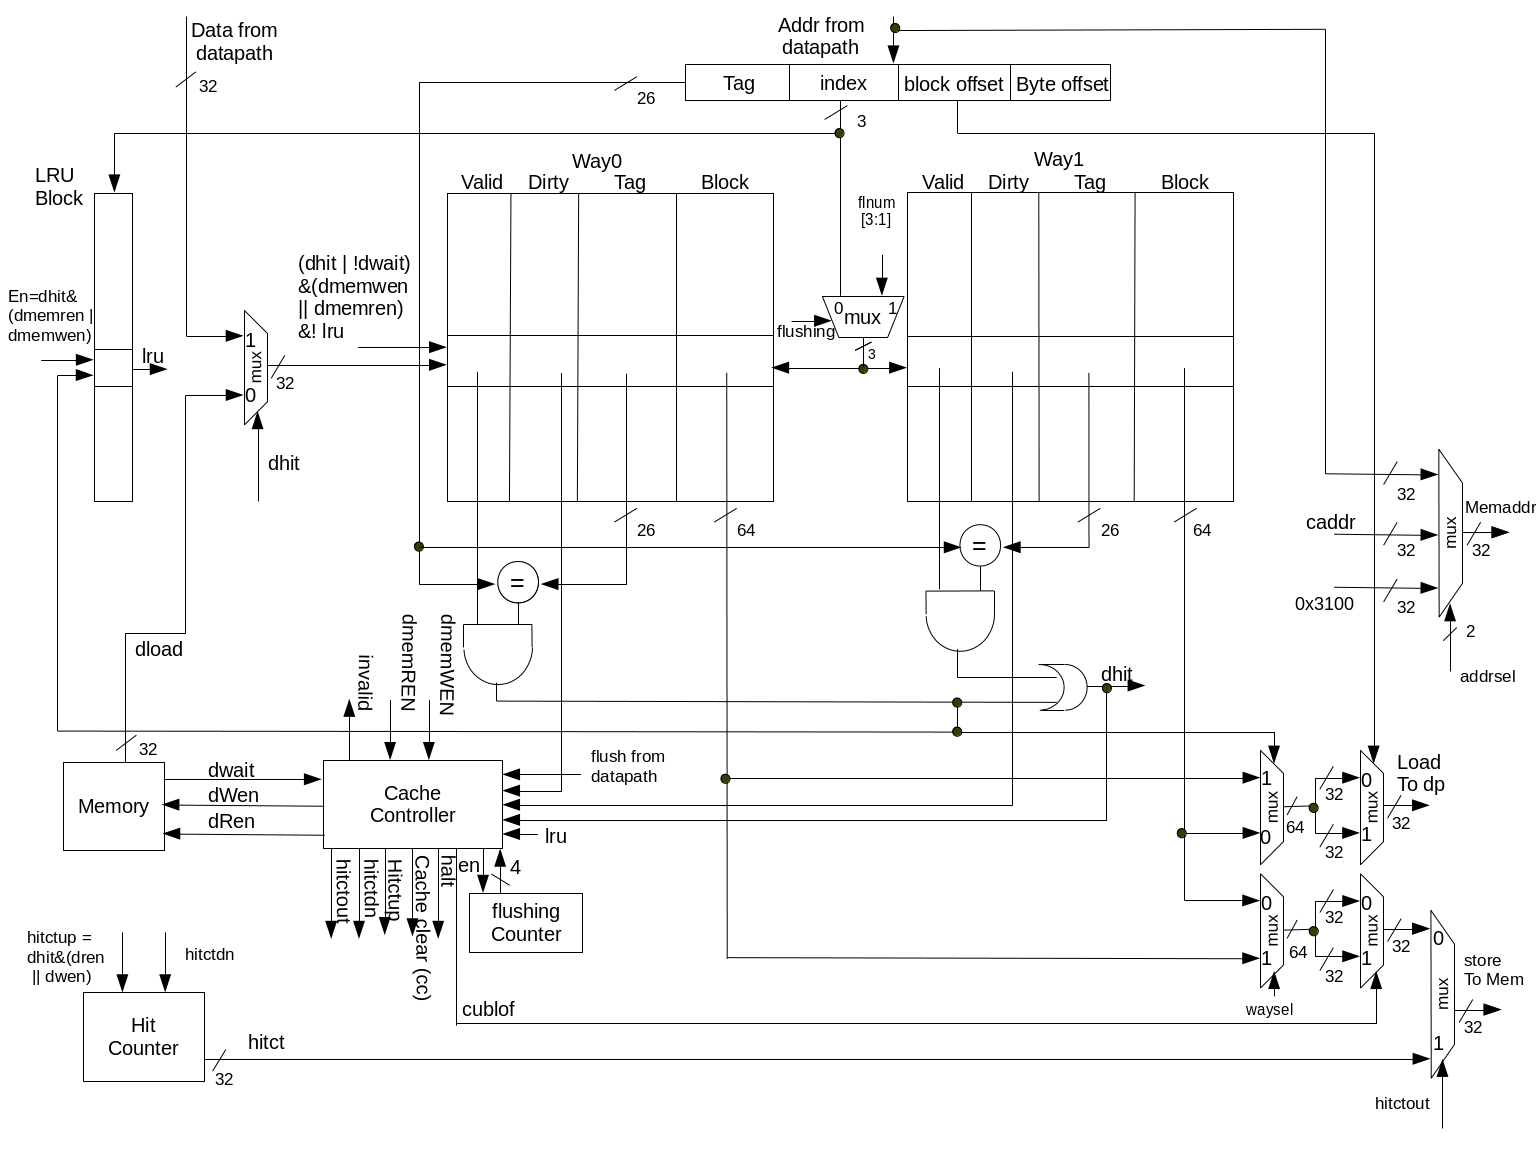
\includegraphics[width=\textwidth]{diagrams/diagram_dcache.png}
    \end{center}

    \caption{Data Cache Block Diagram}
		\label{fig:dcache}
  \end{figure}

% Figure 5. State Diagram of Data Cache
  \newpage
  \begin{figure}[hbp!]
    \begin{center}
      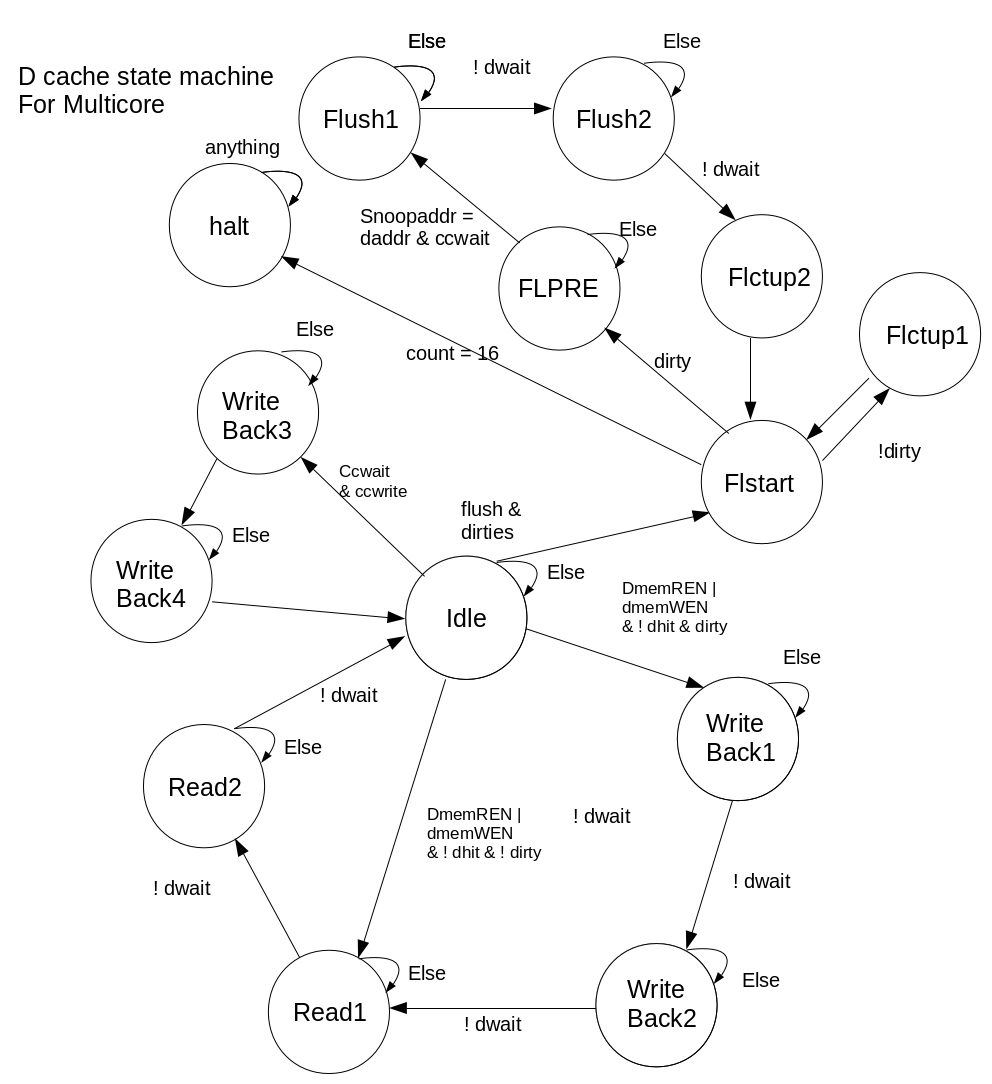
\includegraphics[width=.8\textwidth]{diagrams/dcache_state_machine.png}
    \end{center}

    \caption{Data Cache State Diagram}
		\label{fig:dcache_sd}
  \end{figure}

% Figure 6. Block Diagram and State Diagram of Coherence Control
  \begin{figure}[hbp!]
    \begin{center}
      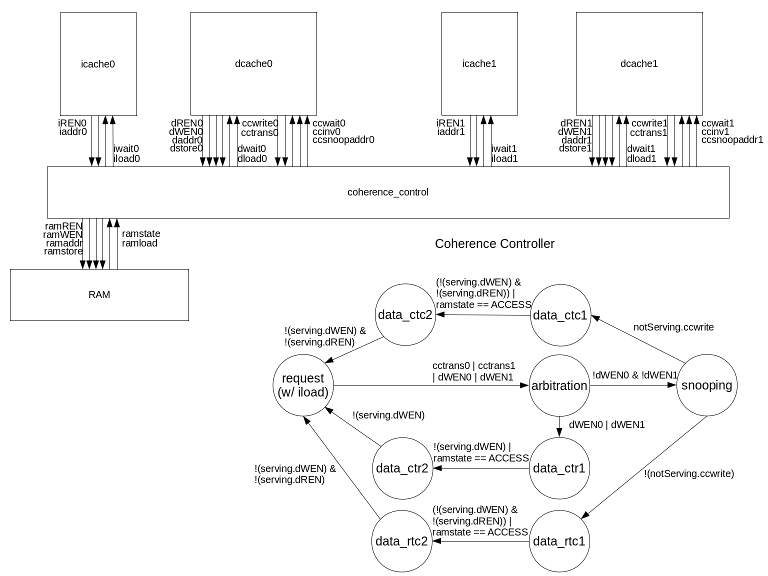
\includegraphics[width=.8\textwidth]{diagrams/diagram_coherence_control.png}
    \end{center}

    \caption{Coherence Control Block Diagram and State Diagram}
		\label{fig:coherence_control}
  \end{figure}

  %Text for discussing your designs in Figure \ref{fig:processor}
  \newpage
  \section{Results}

  \begin{table}[!hbp]
    \singlespacing
    \begin{tabular}{|p{.41\textwidth}|p{.16\textwidth}|p{.16\textwidth}|p{.16\textwidth}|}
      \hline
       & 
      Pipeline\allowbreak Processor\allowbreak without Cache & 
      Pipeline\allowbreak Processor\allowbreak with Cache & 
      Multicore\allowbreak Processor \\ \hline

      Frequency of design: & 63.01 MHz & 42.71 MHz & 31.49 MHz \\ \hline
      Average instructions per clock cycle & 0.6191 & 1.1738 & 1.4441 \\ \hline
      Latency of one instruction & 79.352 ns & 117.069 ns & 158.781 ns \\ \hline
      Total execution time of the program & 1120.24 us & 538.47 us & 595.27 us \\ \hline
      FPGA resources required for design: & -- & -- & -- \\ \hline
      - Total combinational functions & 3521 & 6338 & 13384 \\ \hline
      - Total registers & 2032 & 4470 & 8854 \\ \hline
      Speedup from sequential to parallel & -- & -- & 0.905 \\ \hline
    \end{tabular}

    \caption{Processor Specs}
		\label{tb:procspec}
  \end{table}
  A memory latency of 6 is used for all designs, and a unicore version and a dualcore version of mergesort algorithm are applied. Frequency of design is obtained from the system log which show the restricted Fmax in the ``Slow 1200mV 85C Model Fmax Summary'' section. In this section CLK and CPUCLK frequencies are given and the max possible frequency should be min(CLK/2, CPUCLK). The total number of instructions is obtained from running a ``sim'' command which reports it at the end, and the total clock cycles running the program is obtained from running a ``make system.sim'' command which also reports at the end. The average instruction per clock cycle is (Total number of instructions)/(Total clock cycles). Latency of one instruction is 1/(Max possible frequency) for single cycle processor and 5/(Max possible frequency) for pipeline. Total execution time of the program is (Clock period)*(Total clock cycles). FPGA resources required are found in system FPGA log file in the “Fitter Summary” section. The speedup is calculated by (Execution time of pipeline processor with cache)/(Execution time of multicore processor).

  \section{Conclusion}

  When caches are added to a pipeline processor, extra combinational logic is brought into the design, which elongates the critical path and finally decreases the frequency of the design. The same thing also happens when two cores are brought together with a coherence control added. Thus, the frequency of design keeps dropping. Subsequently, the decrease of frequency results in an increase of latency of one instruction. After caches are added, memory is not accessed when cache hits happen. Accessing caches is much faster than accessing memory; therefore, the average instructions per clock cycle of processor with cache is higher than that of processor without cache. In a multicore processor, programs can be run in parallel, which allow multiple instructions to be executed at a time. So, comparing to a unicore processor, the multicore processor has a higher average instruction per clock cycle. Combining these factors together, the total execution time of the mergesort program decreases from processor without cache to processor with cache, but increases slightly from unicore processor to multicore processor. As a result, the speedup from sequential to parallel is less than 1.\\
  With regards to resource usage, cache design uses almost the same number of combinational logics as datapath, because most of combinational logics in caches have a bus size of a 32-bit word, which dramatically increases the use of gate resources. Multicore design uses nearly double of combinational logics comparing to pipeline with caches design. This result is expected since dual cores need double resources and the coherence control added requires extra logic. Speaking of register usage, most registers in caches design go to cache buffers, others go to cache control state machine and LRU block for efficient cache way selection. Usually caches should use three or four times more registers than datapath, but since we use branch prediction table and some unused instructions are passed through pipeline for debugging, our caches only use twice registers as datapath uses. In conclusion, for our design, one core with caches run fastest among all designs, but if we are able to reduce critical path for multicore design and make it run at faster clock rate, multicore design will have a better performance.

  \section{Contributions}

  Yutong Huang: Data cache and instruction cache block diagram, data cache and instruction cache state machine, data cache implementation, link register logic implementation, datapath integration after adding LL/SC, data cache modification fit to new memory controller, final report overview and part of conclusion.\\
  Yiheng Chi: Instruction cache implementation, data cache and instruction cache test bench, coherence control block diagram, coherence control state machine, coherence control implementation, coherence control test bench, datapath modification for LL/SC, parallel algorithm asm file, final report design, result and part of conclusion.

\end{document}
